% Preamble templated from Mihir-Divyansh/Course-Setup
%iffalse
\let\negmedspace\undefined
\let\negthickspace\undefined
\documentclass[journal,12pt,onecolumn]{IEEEtran}
\usepackage{cite}
\usepackage{amsmath,amssymb,amsfonts,amsthm}
\usepackage{algorithmic}
\usepackage{graphicx}
\usepackage{textcomp}
\usepackage{xcolor}
\usepackage{txfonts}
\usepackage{listings}
\usepackage{enumitem}
\usepackage{mathtools}
\usepackage{gensymb}
\usepackage{comment}
\usepackage[breaklinks=true]{hyperref}
\usepackage{tkz-euclide}
\usepackage{listings}
\usepackage{gvv}
%\def\inputGnumericTable{}
\usepackage[latin1]{inputenc}
\usepackage{color}
\usepackage{array}
\usepackage{longtable}
\usepackage{calc}
\usepackage{multirow}
\usepackage{hhline}
\usepackage{ifthen}
\usepackage{lscape}
\usepackage{tabularx}
\usepackage{array}
\usepackage{float}
\usepackage{caption}
\usepackage{multicol}

\newtheorem{theorem}{Theorem}[section]
\newtheorem{problem}{Problem}
\newtheorem{proposition}{Proposition}[section]
\newtheorem{lemma}{Lemma}[section]
\newtheorem{corollary}[theorem]{Corollary}
\newtheorem{example}{Example}[section]
\newtheorem{definition}[problem]{Definition}
\newcommand{\BEQA}{\begin{eqnarray}}
\newcommand{\EEQA}{\end{eqnarray}}
%\newcommand{\define}{\stackrel{\triangle}{=}}
\theoremstyle{remark}
%\newtheorem{rem}{Remark}

% Marks the beginning of the document
\begin{document}
\bibliographystyle{IEEEtran}
\vspace{3cm}

\title{Assignment 4: 2.9.6}
\author{EE25BTECH11055 - Subhodeep Chakraborty}
\maketitle
\hrulefill
\bigskip

\renewcommand{\thefigure}{\theenumi}
\renewcommand{\thetable}{\theenumi}

\textbf{Question:}\par
$|\vec{a}| = 8, |\vec{b}| = 3, \text{ and } \vec{a}\cdot\vec{b} = 12\sqrt{3}$, then the value $|\vec{a}\times\vec{b}|$ is \par
\textbf{Solution:}\par

Given:
\begin{align}
 \norm{\vec{a}} = 8 \\
 \norm{\vec{b}} = 3 \\
 \vec{a}^\top\vec{b} = 12\sqrt{3}
\end{align}
We know:
\begin{align}
 \norm{\vec{a}\times\vec{b}} &= \norm{\vec{a}}\norm{\vec{b}}\sin\theta \\
 \cos\theta &= \frac{\vec{a}^\top\vec{b}}{\norm{\vec{a}}\norm{\vec{b}}}
\end{align}
Thus
\begin{align}
 \brak{\vec{a}^\top\vec{b}}^2 + \brak{\norm{\vec{a}\times\vec{b}}}^2 = \norm{\vec{a}}^2\norm{\vec{b}}^2
\end{align}
Substituting values
\begin{align}
\norm{\vec{a}\times\vec{b}} &= \sqrt{64\times9-144\times3} \\
\norm{\vec{a}\times\vec{b}} &= 12
\end{align}
\begin{figure}[H]
    \centering
    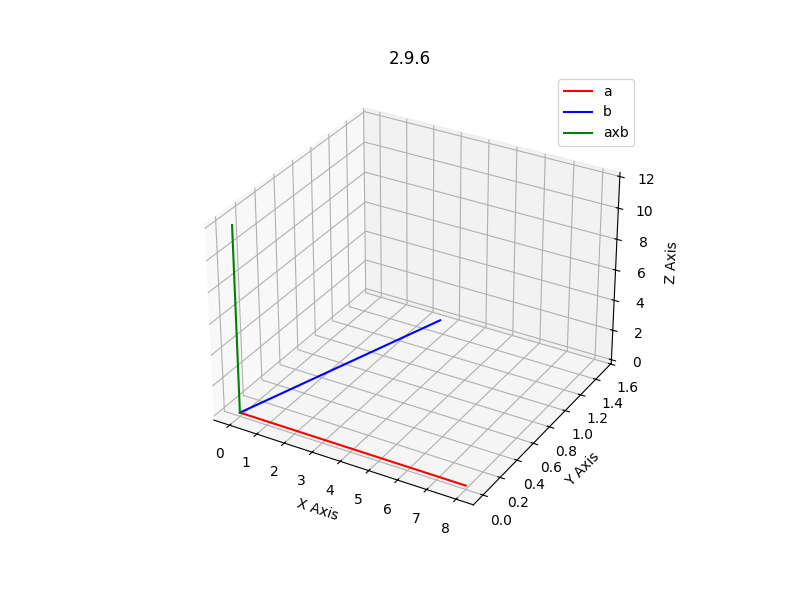
\includegraphics{figs/plot.png}
    \caption*{}
    \label{fig:plot}
\end{figure}
\end{document}
